\newcommand{\upcite}[1]{\textsuperscript{\textsuperscript{\cite{#1}}}}
\documentclass{mcmthesis}
\mcmsetup{
		CTeX = false,
        tcn = 69377,
        problem = D,
        sheet = true, 
        titleinsheet = true, 
        keywordsinsheet = true,
        titlepage = false, 
        abstract = false
}
\usepackage{palatino}
\usepackage{lipsum}
\usepackage{booktabs}
\usepackage{tabu}%%table
\usepackage{colortbl}
\usepackage{indentfirst}%%suojin
\usepackage{geometry}%页面设置  
\usepackage{graphics}%图片设置  
\usepackage{caption}%注释设置  
\usepackage{graphicx}
\usepackage{subfigure}
\usepackage{palatino}
\usepackage{tikz}
\usepackage{enumerate}
\usepackage{longtable}
\usepackage{wrapfig}
\usetikzlibrary{shapes.geometric, arrows}

\title{Fly Through Security Check}
 %正文摘要和控制页摘要名字修改
\def\abstractname{Abstract}
\def\sheetsummaryname{summary}

\begin{document}

 %控制页摘要内容
\begin{sheetsummary}
\par We develop a computer simulation model to identify bottlenecks. We use arrival times and average check time to compute wait time with loops. Results show wait time continue increasing. Finally, we find Zone A and Zone B two bottlenecks. In addition, we develop a queuing model to figure out measures to increase passenger throughput and provide good travel experience. 
\par We mainly propose two modifications to solve the congestion problem at O’ Hare. One is to choose the model of one queue of multiple desks. The other is to change the ratio between number of document checkpoints and security screening equipment.

\par We focus on validating the modifications above. For the first solution, one queue of multiple checkpoints performs better. Average waiting time in Model (Three M/M/1/$\infty$) is 7.5(min). But average waiting time in Model(M/M/3/$\infty$) is 1,89(min). For the second solution, we determine the ratio between number of ID check counters and security equipment according to number of ID checkpoints and security service time. For pre-check passengers, the ratio should be 4: 5. For regular passengers, the ratio should be 4: 8. Finally, we consider the impact of cultural differences on passenger service time. We use the given data as an intermediate value. And we simulate the data of another two travel styles through increasing and decreasing the service speed by 50\%, do a sensitivity analysis and accommodate these differences.
\par Our model is applicable worldwide. In the future we can incorporate the constraints of economic factors to further optimize our model.
\end{sheetsummary}

 %正文摘要内容
\begin{abstract}
\end{abstract}

 %关键词
\begin{keywords}
Queuing Model; Computer Simulation; 
\end{keywords}

\maketitle
 % Generate the Table of Contents, if it's needed.
\tableofcontents
\newpage

%%---------------------------introduction--------------------------------
\section{Introduction}

\subsection{Background}
\par The terrorists attacked the United States on September 11, 2001. Since then, the airport security has been significantly enhanced. Passengers need to remove shoes, belts, jackets, metal objects, and electronic products. They put them in separate X-ray boxes at the airport security checkpoint. The notebooks and some medical equipment also need to be removed from their packs and be placed in separate containers. Because of the lengthy and complex security checkpoints, the passengers wait for too long, or even miss the flights. In order to change the situation that passengers wait too long, the TSA has made some improvements, including some modifications to the checkpoint equipment and the procedures, such as increasing staffs at the airport and introducing a new measure. Approximately $45\%$ of passengers enroll in Pre-Check. They pay $\$85$ to get a background check and enjoy a separate screening process. This change has improved the airport's long wait situation.

\subsection{Our Works}

\begin{itemize}
	\item \textbf{Evaluation model of waiting time}
	\begin{itemize}
		\item \par In the process of the document check, we can use the waiting time of new passengers to describe the flow of people checked by document (when the waiting time for new arrivals increases, which means that the flow of people going through the ID check is low).
		\item \par In the process of the security check, we can use the waiting time of the new arriving passenger who is going to pass the baggage and body screening to describe the flow of people (when the waiting time of additional passenger increases, which means that the flow of people who going through the security check is low)
	\end{itemize}
	\item \textbf{Queuing Theory}
	\par We study the quantity of channels, and different queuing ways to select the reasonable the quantity of channel and the way of queue. Furthermore, we also need to determine the average and variance of the waiting time of customers.
	\item \textbf{Computer Simulation}
	\par Because the subject data is less, not suitable for statistical methods to find data characteristics. Therefore, we establish a recursive algorithm model, make full use of data analysis of passenger queuing time.
	\item \textbf{Multi-objective Optimization Model}
	\par We try to reduce variance in wait time. For increasing passenger throughput, we achieve it also by reducing passengers' average wait time. 
	\par 

	
		
\end{itemize}


%%--------------------------assumptions-------------------------------
\section{Assumptions}

\subsection{About the Given Data}
\begin{itemize}
	\item There is no time for placing items on the belt going into x-ray.
	\item There is no transition time between process stations.
\end{itemize}

\subsection{About Our Model}
\begin{itemize}
	\item Passengers arrive at rate $\lambda$ according to a Poisson process and move the process from state $i$ to $i+1$.
	\item Service times are independent to each other and have an exponential distribution with parameter $\mu$ in the M/M/s queue.
	\item There are $s$ checkpoints ($s$ is a constant), which serve from the front of the queue. If there are less than $s$ passengers, some of the checkpoints will be idle. If there are more than $s$ passengers, they will queue.
	\item There is no limit on the number of passengers wait in line.
	\item Security officers inspect passengers' identification and boarding documents during work time after passengers arrive at the checkpoint. (We will discuss other situations in model modification)
	\item No congestion occur when passengers depart the checkpoint area. 
	\item We use the average passenger wait time to estimate passenger throughput. 
	\item We use the range of passenger wait time at certain probability to measure its variance.
\end{itemize}

%%---------------------------Analysis-problem-----------------------------

\section{Analysis of the Problem}

\par The U.S. Transportation Security Agency (TSA) wants our team to solve the congestion problem at airport. We should mainly consider two aspects: 
\begin{itemize}
	\item Passenger throughput.
	\item Passenger flying experience.
\end{itemize}
\par In order to expedite passenger throughput, we can shorten the time of security check by improve the security process. In terms of passenger flying experience, we try to minimize both the average and variance of waiting time. 

\subsection{Simplification of the Problem}

\par In the process, whether passengers proceed to the conveyor belt on the other side of the X-ray scanner to collect their belongings or they go to Zone D to receive a pat-down inspection because of failure of certain steps, they move forward freely. They do not have to walk in a line. So we do not consider wait time in these two procedures.

\subsection{Analysis of the Process}
\par After our simplification of the problem, we divide the whole process into two parts. In general, passengers will join in two queues and be checked twice.

\begin{itemize}
	\item In the first section, passengers randomly arrive at the checkpoint and wait in a queue until a security officer can inspect their identification and boarding documents.
	\item In the second section, the passengers then move to a subsequent queue for an open screening line. Once the passengers reach the front of this queue, they prepare all of their belongings for X-ray screening. Passengers must remove shoes, belts, jackets, metal objects, electronics, and containers with liquids, placing them in a bin to be X-rayed separately. Laptops and some medical equipment also need to be removed from their bags and placed in a separate bin. Meanwhile the passengers process through either a millimeter wave scanner or metal detector.  
\end{itemize}

\subsection{Solution Steps}

\par We accomplish the task in several steps:
\begin{enumerate}[step 1:]
\item Build a model to review airport security checkpoints and staffing to identify potential bottlenecks that disrupt passenger throughput.
\item Provide solutions that both increase checkpoint throughput and reduce variance in wait time while maintaining the same standards of safety and security.
\item Validate our model by applying our modifications to the current process and demonstrate the changes.
\item Make a sensitivity analysis on how cultural differences may impact the way in which passenger’s process through checkpoints. 
\item Propose policy and procedural recommendations for the security managers based on our model.
\item Assess strengths and weaknesses.
\item Future prospects.
\end{enumerate}


%%-------------------------model---------------------------------------------
\section{Establishment of the Model}

\subsection{M/M/s Waiting Queuing Model}
\subsubsection*{Symbol Description}
\par The common symbols in queuing theory are listed below in table \ref{tab:Symbol Description}.
\begin{table}[h]
\centering
\caption{Symbol Description}\label{tab:Symbol Description}
\begin{tabular}{cc|cc}
\toprule
Symbol & Description & Symbol & Description\\
\midrule
$\lambda$ & the average arrival rate & $L$ & Average team length \\
$\mu$ & the average service rate of a single service & $L_q$ & Average queue length \\
$P$ & the probability of n people in system & $W$ & Average length of stay\\
$n$ & the number of people in system & $W_q$ & Average waiting time\\
\bottomrule
\end{tabular}
\end{table}

\subsubsection*{Queuing system}
\par There are two main queuing system in our model.

\begin{figure}[!h]
\small
\centering
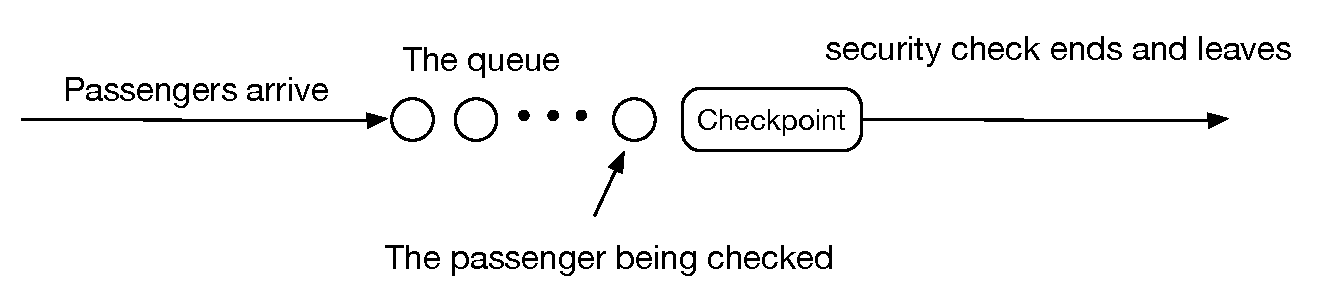
\includegraphics[width=14cm]{1.eps}
\caption{Single-server Queuing System M/M/1} \label{Single-server Queuing System M/M/1}
\end{figure}
\begin{figure}[!h]
\small
\centering
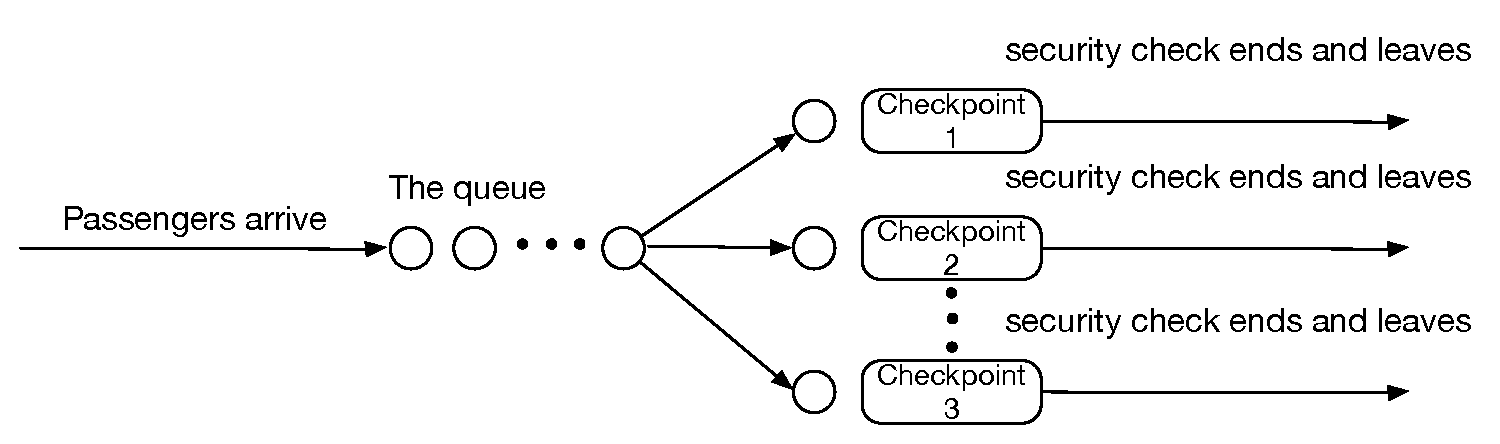
\includegraphics[width=14cm]{2.eps}
\caption{S Parallel Service Desk with One Queuing System M/M/s} \label{S Parallel Service Desk with One Queuing System M/M/}
\end{figure}

\subsubsection*{Birth and Death process}
\par A system of inter-arrival time and service time showed exponential distribution, we denoted M\upcite{1}.
\par Let $E$ represent the number of times of entering state $n$, and $L$ represent the number of times of leaving state $n$. We have $|E-L| \in \{0,1\}$\upcite{1}. When the system arrives at steady state, which means $t$, we have, therefore arrival rate = removed rate.

\subsubsection*{Balance Equation}
\par Three conclusion equations:

\begin{equation}
	C_n = \frac{\lambda_{n-1}\lambda_{n-2}\cdots\lambda_0}{\mu_{n}\mu_{n-1}\cdots\mu_1} \quad (n = 1, 2, \cdots)  \label{C_n}
\end{equation}
\begin{equation}
	P_n = C_n P_0 \quad (n = 1, 2, \cdots)  \label{p_n}
\end{equation}
\begin{equation}
P_0 = {\frac{1}{1+\sum \limits_{n=1}^{\infty} \prod \limits_{i=0}^{n-1}{\frac{\lambda _i}{\mu _{{i+1}}}}}} =\frac{1}{1+\sum\limits_{n=1}^{\infty} C_n} \label{p_0}
\end{equation}

\par Mark $P_n = P\{N = n\} \quad (n = 0,1,2.\cdots)$ as the probability distribution of the queue length $N$ after the system reaches the steady state.

\subsubsection*{Assumprions} 
\begin{itemize}
	\item The passenger arrives alone, and the time interval obeys the negative exponential distribution with the parameter $\lambda$.
	\item Suppose there are $s$ service stations in the system, and the service time of the service desk is independent of each other and obeys the negative exponential distribution with the parameter $\mu$.
	\item Passengers take the initiative to select the free service desk. If there is no free service desk, wait in queue.
\end{itemize}

\subsubsection{Single Desk Model}
\par The single-desk model is the simplest queuing system that we can use it to describe the queuing status of a single security gate.
\par In this model, $\lambda_n = \lambda, n = 1, 2, \cdots$ and $\mu_n = \mu, n = 1, 2, \cdots$ mark $\rho = \frac{\lambda}{\mu}$. And set $\rho < 1$  so that 
$$C_n = \left( \frac{\lambda}{\mu} \right)^n \quad , \quad P_n = \rho^n P_n \quad (n = 1, 2, \cdots) $$
Among them
\begin{equation}
	P_0 = \frac{1}{1 + \sum \limits_{n=1}^\infty \rho^n} = \left( \sum \limits_{n=0}^\infty \rho^n \right)^{-1} = \left( \frac{1}{1 - \rho} \right)^{-1} = 1-\rho
\end{equation}
\par Therefore, the probability value of the number of passengers in the system under equilibrium condition is 
\begin{equation}
	P_n = (1-\rho)\rho^n \quad n = 0, 1, 2, \cdots
\end{equation}
But this equation could obtain only in the condition that $\rho = \frac{\lambda}{\mu} < 1$. 

\subsubsection*{Main Quantitative Indicators}
\par Average team length $L$:
\begin{equation}
			L = \sum \limits_{n = 0}^\infty n P_n = \sum \limits_{n = 1}^\infty n (1 - \rho) \rho^n 
	 	  = \frac{\rho}{1-\rho} = \frac{\lambda}{\mu - \lambda}
\end{equation}
Average queue length $L_q$;
\begin{equation}
\begin{split}
	L_q & = \sum \limits_{n=1}^\infty (n-1)P_n = L - (1 - P_0) \\
	& = L - \rho = \frac{\rho^2}{1-\rho} = \frac{\lambda^2}{\mu(\mu - \lambda)}
\end{split}
\end{equation}
Average length of stay $W$:
\begin{equation}
	W = E(T) = \frac{1}{\mu - \lambda}
\end{equation}
Average waiting time $W_q$:
\begin{equation}
	W_q = W - \frac{1}{\mu} = \frac{\lambda}{\mu(\mu - \lambda)}
\end{equation}

\subsubsection{Multi-service Desk Model}

\par The stationary distribution of queuing systems is discussed below.

\par  For multi-service desk system. There are two equations:$\lambda_n = \lambda \quad n = 0,1,2,\cdots$
and 
$$\mu_n=
\begin{cases}
n\mu & \text{$n = 1, 2,\cdots,s$}\\
s\mu & \text{$n = s, s+1,\cdots$}\\
\end{cases}$$
Mark $\rho_s = \rho/s = \frac{\lambda}{s\mu}$, if $\rho < 1$ , according to equation \ref{C_n} and \ref{p_n}. We have:
\begin{equation}
	C_n = 
	\begin{cases}
		\frac{(\lambda / \mu)^n}{n!} & \text{$n = 1, 2,\cdots,s$}\\
		\frac{(\lambda / \mu)^s}{s!}\left(\frac{\lambda}{s\mu}\right)^{n-s} = \frac{(\lambda / \mu)^n}{s!s^{n-s}} & \text{$n \geqslant s$} \label{C_nMMS}
	\end{cases} 
\end{equation}
So 
\begin{equation}
	p_n = 
	\begin{cases}
		\frac{\rho^n}{n!}p_0  & \text{$n = 1, \cdots, s$}\\
		\frac{\rho^n}{s!s^{n-s}}p_0 & \text{$n \geqslant s$}\\
	\end{cases}
	\label{p_nMMS}
\end{equation}
Among them
\begin{equation}
	p_0 = \left[ \sum \limits_{n=0}^{s-1} \frac{\rho^n}{n!} + \frac{\rho^s}{s!(1-\rho_s)} \right]^{-1} \label{p0MMS}
\end{equation}
\par The probability of the number of passengers in the system under equilibrium is given in equation \ref{p_nMMS} and \ref{p0MMS}. When $n \geqslant s$:
\begin{equation}
	c(s,\rho) = \sum \limits_{n = s}^\infty p_n = \frac{\rho^s}{s!(1-\rho_s)}p_0 \label{csp}
\end{equation}
The equation \ref{csp} is called Erlang Waiting Formula. It gives the probability that a passenger arrives at the system is waiting.


\subsubsection*{Main Quantitative Indicators}
\par Average team length $L$ and average queue length $L_q$:
\begin{equation}
		L  = L_q + \rho \qquad 	L_q  = \frac{p_0\rho^s \rho_s}{s!(1-\rho_s)^2} = \frac{c(s,\rho_s)}{1-\rho_s} 
\end{equation}

Average length of stay $W$ and average waiting time $W_q$: 
\begin{equation}
	W = \frac{L}{\lambda} \qquad W_q = \frac{L_q}{\lambda} = W - \frac{1}{\mu}
\end{equation}



\subsection{Exploration Model by Simulation}
\par Since the amount of data in the data table is too small, we use the simulation method to calculate the sequence of each person's waiting time. 
\par We define the time for the $i_th$ passenger to arrive at the service desk as $T_a(i)$ and the average service time for the service desk to be $T_s$. So that we can get the waiting time $T_w(i)$ of the $i_th$ person.
\begin{equation}
	T_w(i) = T_s + T_w(i-1) + T_a(i-1) - T_a(i)
\end{equation}
\par By analyzing the waiting time data and the arrival time data of each passenger, we can get the distribution of personnel and the bottleneck position in the existing airport security check.

\subsection{Multi-objective Optimization Model}

\par To solve the problem, we should consider both passenger flying experience and passenger throughput. As for passenger flying experience, we aim at minimizing the passengers' average waiting time. \textbf{Meanwhile, we also try to reduce variance in wait time. For increasing passenger throughput, we achieve it also by reducing passengers' average wait time. Here we explain the principle.} We use average arrival time interval to calculate the speed of passengers' arrival. Similarly, we utilize average security check time to estimate the speed of security check. When average arrival time interval is equal to average security check time, we say there is a balance between passengers' arrival and security check, so the average wait time remains the same. However, if passengers' average wait time is shorter, in condition of the same speed of passengers' arrival, the speed of security check must be higher. In situation where passengers queue in line in most of the time, passenger throughput heavily depends on the speed of security check in a positive correlation. So if we take measures to successfully reduce passengers' average wait time, we also improve passenger throughput. Meanwhile, we provide a better passenger experience. 
\par So after problem conversion, we are actually concerned with passengers' average wait time as well as variance in it. Our goal is to optimize the two targets simultaneously.
\subsection*{Model Application in Reality}
\par In the situation, passengers arrive at airport when officers are at work. However, in reality, there are already some people waiting in line when officials begin with security check. So the actual average passenger wait time equals to the sum of the ideal average passenger wait time and time of security check for passengers in front of them.
%%---------------------------------------------------------------

\section{Calculation and Analysis of the Model}
\subsection{Task A}
\par To deal with task a, we use our exploration model by computer simulation to explore the flow of passengers through a security check point and identify bottlenecks. We use the given data to complete the task. Although each column of data in the dataset is independent of the others as the data were collected as several groups of people were coming through the screening process, we can obtain some information such as average time of document check process, millimeter wave scan and X-Ray scan. Furthermore, we develop a simulation model to make full use of the data. We get data of wait time for every passenger in Column A and B for further analysis. In particular, we interpret data in these ways:
\begin{itemize}
	\item We combine Column C and Column D to calculate the average time of Document check.
	\item We divide data in Column H(time to get scanned property) into two groups in ascending order of time. We consider the 45 percent data in the front come from pre-check passengers because approximately $45\%$ of passengers enroll in the pre-check program. 
\end{itemize}

\begin{figure}[htbp]  
\begin{minipage}[t]{0.5\textwidth}
\centering  
\includegraphics[width=\linewidth]{TSA.png} \\
X-axis values = arrival order\\
Y-axis values = time the people wait (s).
\caption{TSA Pre-check Wait Time} \label{TSA Pre-check Wait Time}
\end{minipage}
\hspace{1ex}
\begin{minipage}[t]{0.5\textwidth}  
\centering  
\includegraphics[width=\linewidth]{PAX.png}\\
X-axis values = arrival order\\
Y-axis values = time the people wait (s).
\caption{Regular Pax Wait Time}  \label{Regular Pax Wait Time}
\end{minipage}  
\end{figure} 


\begin{figure}[h]
\small
\centering
\includegraphics[width=12cm]{step2.png}\\
X-axis values = arrival order\\
Y-axis values = time the people wait (s).
\caption{Baggage and Body Screening} \label{fig:Baggage and Body Screening}
\end{figure}

\par We can see the passenger wait time in the figure\ref{TSA Pre-check Wait Time} and figure \ref{Regular Pax Wait Time} is continuously increasing. In other words, document checkpoints are congested because the arrival speed is faster than the speed of document check. So we identify document checkpoint as a bottleneck. We apply the same method to analyze baggage and body screening (showed figure \ref{Baggage and Body Screening}), and get the similar conclusion. However, the trend of rising up is more obvious compared to document check. Therefore, baggage and body screening checkpoint is another bottleneck we identify.

\subsection{Task B}
\par We develop five potential modifications to the current process to improve passenger throughput and reduce variance in wait time. We model these changes to demonstrate the impact of our modification. Each modification is followed by corresponding validation. 
\subsubsection*{Modification 1} 
\par \textbf{Method}
\par We can increase the quantity of document Checkpoints to 8. document Check makes no difference for pre-check passengers and regular passengers. Given the number of pre-check passengers (45\%) is approximately equal to the number of regular passengers (55\%), it is reasonable to set 4 as the quantity of document checkpoints for both pre-check passengers and regular passengers. 
\par \textbf{Principle}
\par With other conditions unchanged, when we increase the number of security checkpoints, we can reduce the average passenger wait time. When we have only one checkpoint, we cannot apply M/M/1 model because the speed of document check is slower than the speed of passenger arrival. No balance will be achieved in this condition. We cannot use the former formula in the queuing theory, either. So we use the data given in the excel sheet to calculate the average waiting time of the customer by simulation, the method we have explain before.

\par \textbf{Verification}
\par The first column in the chart is based on the data presented in the table and we calculate the average passenger wait time. We find that the average passenger wait time is long, meanwhile the passenger throughput is low.
\par The second column in the chart shows the result of our multi-service-based queuing model. We select two document checkpoints, and the average passenger wait time (pre check) is 7.5 seconds compared to the first one we calculated. The average wait time in this model is significantly shorter. So we believe that the passenger throughput increases. And the probability of the longest passenger wait time less than 33 seconds is 95\%. So the passenger wait time range is relatively large.
\par The third column in the chart shows the result of our multi-service-based queuing model. Now, we choose three document checkpoints. And the average passenger wait time we calculate is 0.99 second. Compared with the previous two results we calculate, the average waiting time has a noticeable shortening of the time. That is to say, the passenger throughput increases. And the probability of the longest waiting time less than 7 seconds is 95\%. Comparing the 2 longest passenger wait time, we can see variance of wait time reduce.
\par The fourth column in the chart shows the result of our multi-service-based queuing model. At this time, we choose four document checkpoints. And the average passenger wait time is 0.17second. Compared with the three results we calculated, the average waiting time has a noticeable shortening of the time. In others words, we believe that the passenger throughput increases. And the probability of the longest waiting time less than 0.2 second is 95\%. Comparing the 3 longest passenger wait time, we can see variance of wait time.
\par When we continue to increase the number of document checkpoints,there is no obvious decrease in average passenger wait time. 
\par So when we increase the number of document checkpoints, we can increase the flow.
\par Comparing the results obtained by simulation with another three different model in the queuing theory: M/M/2, M/M/3 and M/M/4(showed in table \ref{Modification 1}), we arrive at a conclusion that when the number of security checkpoints is increased, the average wait time of passengers will be greatly reduced, eventually, passenger throughput of the airport will be increased. 
\begin{table}[h]
\centering
\caption{Comparing Data}
\label{Modification 1}
\begin{tabular}{l|c|c|c|c}
\toprule
Item  & $s=1$  & $s=2$   & $s=3$   & $s=4$ \\                      
\midrule
Average team length $L$ ($people$)         &  -& 2.04 & 1.36 &1.27\\
          
Average queue length $L_q$ ($people$)      &   -& 0.79 & 0.11 &0.02\\        
Average length of stay $W$ ($s$)           &  -& 18.39 & 12.23 &11.41\\   
Average waiting time $W_q$ ($s$)           & 51.048  & 7.15 & 0.99 & 0.17 \\
Service Desk Usage $\rho$                  &   -& 0.62 & 0.42 & 0.31\\ 
$95\%$ reliability maximum time ($s$)      &    106.9  & 33 & 7 & 0.2\\         
\bottomrule        
\end{tabular}
\end{table}

\par \textbf{Conclusion}
\par At the same time, we can get the probability of wait time in a certain range. The probability can measure variance in passenger wait time. In other words, we can obtain the range of wait time on condition of a given probability. We choose the probability to be 95\% to calculate the range of passenger wait time for later comparison. 

\subsubsection*{Modification 2}
\par \textbf{Method}
\par One queue of multiple checkpoints performs better.
\par \textbf{Principle}
\par According to the "Queuing Theory", we have two methods of queuing. The one is M/M/S model of queuing. In others words, passengers wait in line as soon as they arrive, and they go to the free document checkpoint one by one. The other is $s \times M/M/1$. $s \times M/M/1$ is the method of queuing that passengers can choose any one of document checkpoint.
\par \textbf{Verification}
\par We use a simple example to compare the two models as follow.
\par The security checkpoint has three document checkpoints. The average passenger arrival rate $\lambda = 0.9person/min$; Average service rate at the checkpoint $\mu = 0.4 $$ person/min$.
\par The queuing problem is analyzed using the M/M/s/$\infty$ and M/M/1/$\infty$ models, respectively, and get the results table\upcite{2}.Through the following table \ref{compareTable}, we understand If the number of service desk and service rate unchanged, the single team queuing way better than the multi-team queuing.
\begin{table}[!htb]
\centering
\caption{The Result Table}
\label{compareTable}
\begin{tabular}{@{}c|c|c@{}}
\toprule
Item                                         & M/M/3/$\infty$                    & Three M/M/1/$\infty$                        \\ \midrule
Idle probability                             & \cellcolor[HTML]{9AFF99}0.0748    & \cellcolor[HTML]{FFFC9E}0.25 Each subsystem \\
The probability that the passenger must wait & \cellcolor[HTML]{9AFF99}0.57      & \cellcolor[HTML]{FFFC9E}0.75                \\
Average team length                          & \cellcolor[HTML]{9AFF99}3.95      & \cellcolor[HTML]{FFFC9E}9 Whole system      \\
Average queue length                         & \cellcolor[HTML]{9AFF99}1.70      & \cellcolor[HTML]{FFFC9E}2.25 Each subsystem \\
Average length of stay                       & \cellcolor[HTML]{9AFF99}4.39(min) & \cellcolor[HTML]{FFFC9E}10(min)             \\
Average waiting time                         & \cellcolor[HTML]{9AFF99}1,89(min) & \cellcolor[HTML]{FFFC9E}7.5(min)  \\
\bottomrule        
\end{tabular}
\end{table}
\par \textbf{Conclusion}
\par By comparing 2 methods of queuing,We know that one queue of multiple checkpoints performs better.

\par So that we choose figure\ref{S Parallel Service Desk with One Queuing System M/M/1} to be our queuing model.


\subsubsection*{Modification 3}
\par \textbf{Method}
\par Optimize the ratio of the number between the security check equipment (including the millimeter scan and X-ray scan) and document checkpoints to 5:4.
\par \textbf{Principle}
\par We apply the statistical analysis to the original process. When the number of the document checkpoints is equal to that of security inspection equipment, the average passenger wait time for document check is less than that for baggage and body security. The average passenger wait time depends on the time the person pass the millimeter wave body scanner as well as the time the item is scanned. We can shorten the average passenger wait time for baggage and body screening by increasing the number of security check equipment (showed in table \ref{Modification 3-1} and \ref{Modification 3-2}).

\par \textbf{Verification}
\par The figure shows the average passenger wait time for document check and baggage and body screening. By comparing the average length of time, we select one with the shortest average passenger wait time. In order to make the ratio of the average passenger wait time close to 1, we determine the ratio of the number between baggage and body screening and document check to be 5:4. We can also observe that when the ratio between the two is 5:4, for example 4 security check ports and 5 sets of security equipment, the variance range of average passenger wait time at the possibility of 95 percent is very small. 
\begin{table}[h]
\centering
\caption{Regular Pax Data Sheet}
\label{Modification 3-1}
\begin{tabular}{@{}l|c|ccccl@{}}
\toprule
\multicolumn{1}{c|}{Regular Pax}      & Document Check & \multicolumn{5}{c}{Baggage and Body Screening} \\ \midrule
\multicolumn{1}{c|}{Item}             & $s=4$          & $s=4$   & $s=5$   & $s=6$   & $s=7$   & $s=8$   \\ \midrule
Average team length $L$ ($people$)    & 0.89           & 6       & 3.83    & 3.24    & 3.31    & 3.27    \\
Average queue length $L_q$ ($people$) & 0              & 2.74    & 0.57    & 0.16    & 0.05    & 0.01    \\
Average length of stay $W$ ($s$)      & 11.29          & 68.2    & 43.53   & 38.88   & 37.58   & 37.2    \\
Average waiting time $W_q$ ($s$)      & 0.05           & 31.17   & 6.49    & 1.84    & 0.55    & 0.16    \\
Service Desk Usage $\rho$             & 0.22           & 0.81    & 0.65    & 0.54    & 0.47    & 0.41    \\
$95\%$ reliability maximum time ($s$) & 0.1            & 123     & 40      & 13      & 1       & 0.2     \\ \bottomrule
\end{tabular}
\end{table}


\begin{table}[h]
\centering
\caption{TSA Pre-Check Data Sheet}
\label{Modification 3-2}
\begin{tabular}{@{}l|c|cccc@{}}
\toprule
\multicolumn{1}{c|}{TSA Pre-Check}    & Document Check & \multicolumn{4}{c}{Baggage and Body Screening} \\ \midrule
\multicolumn{1}{c|}{Item}             & $s=4$          & $s=2$      & $s=3$      & $s=4$     & $s=5$     \\ \midrule
Average team length $L$ ($people$)    & 1.27           & 3.36       & 1.72       & 1.54      & 1.5       \\
Average queue length $L_q$ ($people$) & 0.02           & 1.87       & 0.23       & 0.04      & 0.01      \\
Average length of stay $W$ ($s$)      & 11.41          & 38.19      & 19.58      & 17.44     & 17.04     \\
Average waiting time $W_q$ ($s$)      & 0.17           & 21.24      & 2.63       & 0.5       & 0.1       \\
Service Desk Usage $\rho$             & 0.31           & 0.75       & 0.5        & 0.37      & 0.3       \\
$95\%$ reliability maximum time ($s$) & 0.2            & 82         & 17         & 2         & 0.1       \\ \bottomrule
\end{tabular}
\end{table}
\par \textbf{Conclusion}
\par To obtain the largest passenger throughput, we need to make the ratio of number between security check equipment and document checkpoints to be 5:4. In this condition, we can also ensure the average passenger wait time remain a low value, which benefits the passengers.






\subsubsection*{Modification 4}
\par \textbf{Method}
\par Technology brings us new check methods, such as face recognition. Face recognition greatly shortens the average service time in document checkpoints. So we can reduce the average passenger waiting time in document checkpoints.
\par \textbf{Principle}
\par The average service time of face recognition is shorter than the average service time of document checkpoints. So we can reduce the average passenger waiting time in document checkpoints.
\par \textbf{Verification}
\par When we use face recognition, the average passenger wait time of document check is 0.12 second, and the probability of the longest passenger wait time less than 1 second is 95\% (showed in table \ref{Modification 4}) while the average waiting time of document check without facial recognition is 7.15s, and the probability of the longest passenger wait time less than 33 second is 95\% .It can be seen that the mean waiting time reduces. That is to say, the passenger throughput increases, and the variation of the wait time reduces.

\begin{table}[h]
\centering
\caption{Document Check by Face Recognition}
\label{Modification 4}
\begin{tabular}{c|l|c}
\toprule
 &\multicolumn{1}{c|}{Item}  & $s=1$  \\                      
\midrule
\multirow{6}{*}{TSA Pre-Check}
&Average team length $L$ ($people$)         & 0.12 \\
          
&Average queue length $L_q$ ($people$)      & 0.01 \\        
&Average length of stay $W$ ($s$)           & 1.12 \\   
&Average waiting time $W_q$ ($s$)           & 0.12 \\
&Service Desk Usage $\rho$                  & 0.11 \\ 
&$95\%$ reliability maximum time ($s$)      & 1 \\ 
\midrule
\multirow{6}{*}{Regular Pax}
&Average team length $L$ ($people$)         & 0.09 \\
          
&Average queue length $L_q$ ($people$)      & 0.01 \\        
&Average length of stay $W$ ($s$)           & 1.09 \\   
&Average waiting time $W_q$ ($s$)           & 0.09  \\
&Service Desk Usage $\rho$                  & 0.08 \\ 
&$95\%$ reliability maximum time ($s$)      & 0.4 \\        
\bottomrule        
\end{tabular}
\end{table}

\par \textbf{Conclusion}
\par Replace the traditional inspection method with the new inspection equipment, such as Face recognition.


\subsubsection*{Modification 5}
\par \textbf{Method}
\par Encourage more people to participant in Pre-check.
\par \textbf{Principle}
\par Pre-check will not greatly shorten the average waiting time of passengers. But it plays an important role in the baggage and body screening. Because the Pre-check are not required to remove shoes, belts, or light jackets, and they also do not need to remove their computers from their bags. So they save a lot of time. That is to say the waiting time of queuing in the security check phase is shorter than the average waiting time of the general queue, and the change of the waiting time is smaller.
\par \textbf{Verification}
\par Take the example of open queues with 4 security check. As for the Pre-check passenger, the average passenger wait time is 0.5 second, and the probability of the longest passenger wait time less than 2 seconds is 95\%; While the average ordinary passenger waiting time is 31.17 seconds, and the probability of the longest passenger wait time less than 123 seconds is 95\%. We can know that the average passenger wait time is reduced, that is, the throughput increases, and the variation of the waiting time reduces.
\begin{table}[h]
\centering
\caption{Data Compare}
\label{Modification 5}
\begin{tabular}{@{}l|c|c@{}}
\toprule
\multicolumn{1}{c|}{}                 & \multicolumn{2}{c}{Baggage and Body Screening} \\ \midrule
\multicolumn{1}{c|}{Item}             & Regular Pax $s=4$     & TSA Pre-Check $s=4$     \\ \midrule
Average team length $L$ ($people$)    & 1.54                  & 6                       \\
Average queue length $L_q$ ($people$) & 0.04                  & 2.74                    \\
Average length of stay $W$ ($s$)      & 17.44                 & 68.2                    \\
Average waiting time $W_q$ ($s$)      & 0.5                   & 31.17                   \\
Service Desk Usage $\rho$             & 0.37                  & 0.81                    \\
$95\%$ reliability maximum time ($s$) & 2                     & 123                     \\ \bottomrule
\end{tabular}
\end{table}




\par \textbf{Conclusion}
\par More people being participant in Pre-check will reduce the average passenger wait time and increase the passenger throughput.




\subsection{Task C}
\textbf{Method}
\par All over the world, different areas have different cultural norms that shape the local rules of social interaction. In general, people tend to form certain characters because of their local cultural influence. Some people may pay more attention to efficiency, whereas others do not attach much importance to it. In this specific example, some passengers expect to pass security check as quickly as possible. If they happen to choose regular check points, then they will try to speed up during the process. They tend to do things such as removing shoes, belts, jackets, metal objects, electronics, and containers with liquids more quickly. However, others’ action may be slower. Therefore, cultural differences may impact the serve time in which passenger’s process through checkpoints. We simulate three traveler styles, using the data searched from Beijing International Airport as the middle one. And we generate data of another two traveler styles by increasing and decreasing 50\% the speed of the middle. 
\par According the data we searched, the T3 terminal has 30 security checkpoints. It is designed to send up to 3215 passengers per hour. And annual throughput is 17500000 every year.Meanwhile Beijing International Airport usually opening only $1/3$ of the security gate\upcite{3}.
\par So that we get some effective value for queue theory: $\lambda = 0.0298$ and $\mu = 0.0331$.
\par \textbf{Result}
\par In order to accommodate these differences in a manner that expedites passenger throughput and reduces variance the security system, we can change the number of checkpoints based on task B. The sensitivity analysis result is showed in the following figure. See the appendix for more details about the calculation results.
\begin{figure}[h]
\small
\centering
\includegraphics[width=12cm]{taskc.png}\\
X-axis represents the average inspection time.\\
Y-axis represents the checkpoint number need to open\\
\caption{The Balance between Checkpoints Number and Average Check Time} \label{fig:The Balance between Checkpoints Number and Average Check Time}
\end{figure}

\section{Strengths and Weaknesses}
\subsection{Strengths}
\begin{itemize} 
\item \textbf{We make full use of the data and conditions given by the question and analyze carefully.}
\par Particularly, we develop an exploration model by computer simulation to calculate the average passenger wait time. By detecting the trend of the average passenger wait time, we can easily identify bottlenecks.
\item \textbf{Our model is strongly supported by queuing theory.}
\par As a traditional theory, queuing theory has a wide range of application, which has been successfully validated.

\item \textbf{We simplified steps and models after rational analysis.} 
\par By proper problem conversion, we use the average passenger wait time to estimate passenger throughput. And we use the range of passenger wait time at certain probability to measure its variance.
\end{itemize}
\subsection{Weaknesses}
\begin{itemize}
	\item We don’t take the economic factors into consideration and we ignore the airport’ profits due to lack of data.
	\item We assume passengers arrive at rate $\lambda$ according to a Poisson process. However, we ignore the impact of unexpected factors on queuing time at airport.
\end{itemize}


\section{Future Work}
\subsection*{A Multi-objective Programming Model Considering Economic and queuing Factors}

\par In general, increasing the quantity and quality of services can reduce customer waiting costs. But it will also increase the cost of service agencies. Take the case of airports for example, the cost of airports will be increased when the airport increases the opening of the security checkpoints, and the cost of the airport will also increase when the ratio of airport security equipment is increased. One of the objectives of the optimization is to minimize the costs of both service agencies and passengers and determines the level of service to achieve the optimal goal.
\par So the future research direction that we are going to study is that we need to take   economic factors into consideration. Then, we build the model to make the economic factors, the airport throughput, the average passenger wait time to achieve optimal at the same time.

\subsection*{Other Ways to Measure Variance in the Average Passenger Wait Time}
\par Usually, it is not enough to use only one index to measure variance in the average passenger wait time. Here we come up with two more ways for estimation.
\par The first one is to directly calculate the variance. If the value is large, then it means the change is acute. However, this method will work only when you have considerable amount of data. Otherwise, the results will not be reliable nor convincing.
\par The second method imitates the definition of travel time index\upcite{5} - the ratio of travel time in the peak period to the travel time at free-flow conditions. A value of 1.30 indicates a 20-minute free-flow trip takes 26 minutes in the peak period. Similarly, we can define an index C as the quotient of peak passenger wait time divided by average passenger wait time. The value of C not only indicates the intensity of congestion, but also suggests the ability of the security system to accommodate towards stability is poor.
\section{Policy and Procedural Recommendations}

\par After the analysis of airport congestion, we establish our simulation and queuing models to solve the problem.  Our policy and procedural recommendations cover the sequence of airport security check and the number of security checkpoints. We propose them based on the information we obtain such as the average check time of each kind and average passenger wait time for different categories of security check.
\subsection*{Recommendation}
\begin{enumerate}[1:]
\item Encourage more people to enroll in pre-check program.
\item Increase the number of document checkpoints at airport. (4 checkpoints for pre-check passengers, 4 checkpoints for regular passengers)
\item change the queuing form to a queue of multi-service
\item Use the actual time of document check and baggage and body screening time to determine the ratio of the number between document checkpoints and screening equipment. (the ratio should be 4:5 for pre-check passengers while it should be 4:8 for regular passengers)
\item Apply advanced technology. For instance, replace the traditional inspection method (traditional document check) with the new inspection equipment, like face recognition.	
\end{enumerate}

\par In particular, we provide some proposals based on the data we get from the excel dataset. In the situation, we assume the sum of the average security check in each period to estimate the total average time of security check. we should encourage more people to enroll in pre-check program, thus greatly shortening the time of security time. At the same time, we should make the ratio of the number between people participate in the pre-check program and passengers who go through regular process correspond with the ratio of the number between pre-check security checkpoints and regular checkpoints that are opened. We open the number of security mouth for a total of 8 (4 checkpoints for pre-check passengers, 4 checkpoints for regular passengers), which can reduce the average passenger wait time for the two types of passengers waiting to pass document check. We use a queue of multi-service mode of service, which offer another way to decrease the average passenger wait time. For pre-check passengers, we determine the ratio of the number between document checkpoints and security check equipment ratio as 4:5. So we open four document checkpoints for pre-check passengers. Correspondingly, we open four document checkpoints for regular passengers, which means we should be equipped with five sets of security equipment. Similarly, the opening of four regular document checkpoints requires the optimization of 8 sets of security equipment. The new ratio ensures that the average passenger wait time in the whole queuing phase is relatively low and the variation of average passenger wait time is small.





































\begin{thebibliography}{99}

\bibitem{1} \url{https://en.wikipedia.org/wiki/Queueing_theory#Example_of_M.2FM.2F1}
\bibitem{2} \url{http://www.supositorio.com/rcalc/rcalclite.htm}
\bibitem{3} \url{http://news.syd.com.cn/system/2013/08/13/010136939.shtml}
\bibitem{4} \url{http://www.supositorio.com/rcalc/rcalclite.htm}
\bibitem{5} \url{http://d2dtl5nnlpfr0r.cloudfront.net/tti.tamu.edu/documents/ums/congestion-data/national/national-table1.pdf}
\end{thebibliography}








\begin{appendices}
\par Here are two tables.
\par Table 1 is a collection of data for Task C, which describes how the average waiting time is stabilized by adjusting the number of security channels at different security times.
\par Table 2 is the raw data through computer simulation of the waiting time set.
\begin{figure}[h]
\small
\centering
Table 1
\includegraphics[width=12cm]{data2.png}
\end{figure}
    
\begin{figure}[h]
\small
\centering
Table 2\\
\includegraphics[width=14cm]{data.png}
\end{figure}


\end{appendices}

\end{document}

